\documentclass{article}

\usepackage{../preamble}
\standalonetrue

\pagestyle{fancy}
\fancyhf{}
\rhead{Section \thesection}
\lhead{MATH 316 Lecture 14}
\rfoot{Page \thepage}


\title{MATH 316 Lecture 14}
\author{Ashtan Mistal}
\date{June 7, 2021}

\begin{document}

\ifstandalone
\maketitle
\fi

\graphicspath{{./Lecture14/}}

Notes about the midterm:

\begin{itemize}
    \item Format is the same as the practice exams available on Professor Pierce's page
    \item You will get a pdf file with the questions and you can hand-write / use a tablet, etc. 
    \item We will have around an hour to write. 
    \item Closed book, zoom invigilation. You are allowed nonscientific calculators. 
\end{itemize}

\section{Laplace equations}

Last time, we discussed the D'Alembert solution to the wave equation, and we learned how it is relevant to the separation of variables solution. We also discussed characteristics, domain of dependence, and region of influence. We also did some examples, then proceeded to introduce the Laplace equation. The Laplace equation ($ \Delta u = 0, \quad \frac{\partial^2 u}{\partial x^2} + \frac{\partial^2 u}{\partial y^2} = 0$) resulted in being the steady-state of the heat equation, which we solve using separation of variables method by breaking a complex problem (4 inhomogeneous boundary conditions) into building blocks\footnote{For each problem, we would get one inhomogeneous boundary condition and 3 homogeneous, which we use separation of variables for. }. 

\subsection{Example 12}

$$\Delta u = 0$$

$$u(0,y) = 0, \quad u(a,y) = 0, \quad \text{for } y \in [0,b]$$

$$u(x,0) = f(x), \quad u(x,b) = 0 \quad \text{for } x \in [0,a]$$

We have only one inhomogeneous boundary condition ($f(x)$). First, let's sketch the domain and boundary condition:
\begin{center}
    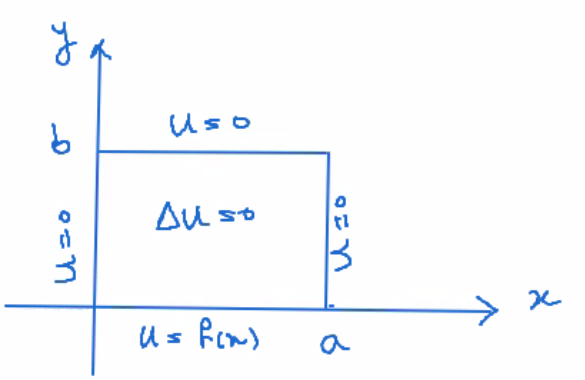
\includegraphics[width = 0.6 \textwidth]{image1.png}
\end{center}

$$u(x,y) = X(x) Y(y) \Rightarrow \frac{X''}{X} = - \frac{Y''}{Y} = - \lambda$$

Now, for the boundary conditions:

$u(0,y) = 0 \Rightarrow X(0) = 0$, $u(a,y) = 0 \Rightarrow X(a) = 0$, and $X'' + \lambda X = 0$. Hence, this is a P1 problem. 

$$\Rightarrow \lambda_n  \left( \frac{n \pi}{a} \right)^2 \quad \text{for } n = 1,2,3$$


$$X_n(x) = \sin \left( \frac{n \pi x}{a} \right)$$

Problem for $Y(y)$:

$$Y_n '' - \lambda_n Y_n = 0$$

Notice the sign change for $\lambda$.


$$Y_n(y) = C_1 e^{\frac{n \pi y}{a}} + C_2  e^{\frac{- n \pi y}{a}}$$

$$u(x,b) = 0 \Rightarrow Y(b) = 0 \Rightarrow C_2 = - C_1 e^{\frac{2 n \pi b}{a}}$$

\begin{center}
    Therefore, $Y_n (y) = C_1 \left[ e^{\frac{n \pi y}{a}} - e^{ \frac{n \pi}{a} (2b-y)} \right]$
\end{center}
 
 $$ = 2 C_1 e^{\frac{n \pi}{a} b} \left[ \frac{e^{ \frac{n \pi}{a} (y-b)} - e^{- \frac{n \pi}{a} (y-b)}}{2} \right]$$
 
 This can be written in terms of $\sinh()$:
 
 $$ = d_1 \sinh \left( \frac{n \pi}{a} (y-b) \right)$$
 
$$\Rightarrow u_n (x,y) = \sin \left( \frac{n \pi}{a} x \right) \sinh \left( \frac{n \pi}{a} (y-b) \right)$$

This satisfies the PDE, and 3 out of 4 boundary conditions. (Why only 3? We haven't substituted the inhomogeneous boundary condition yet). 

Now, we superimpose the eigensolutions. 

$$u(x,y) = \sum_{n=1}^\infty d_n u_n (x,y) = \sum_{n=1}^\infty d_n  \sin \left( \frac{n \pi}{a} x \right) \sinh \left( \frac{n \pi}{a} (y-b) \right)$$

Given we have $u(x,0) = f(x)$, we want to write $f(x)$ in terms of a Fourier sine series. 

$$u(x,0) = f(x) = - \sum_{n=1}^\infty d_n \sin \left( \frac{n \pi}{a} x \right) \sinh \left( \frac{n \pi}{a} (y-b) \right)$$

Given sinh is an odd function. 

If we write $f(x)$ as a fourier sine series, we get:

$$f(x) = \sum_{n=1}^\infty b_n \sin \left( \frac{n \pi x}{a} \right)$$

Match up the coefficients:

$$\Rightarrow - d_n \sinh \left( \frac{n \pi}{a} b \right) = b_n \quad \Rightarrow d_n = \frac{- b_n}{\sinh \left( \frac{n \pi}{a} b \right)}$$

Finally, we get the following:

$$u(x,y) = - \sum_{n=1}^\infty \frac{ b_n}{\sinh \left( \frac{n \pi}{a} b \right)} \sin \left( \frac{n \pi}{a} x \right) \sinh \left( \frac{n \pi}{a} (y-b) \right)$$

\subsection{Example 13}

How about a $u_w$ problem?

\begin{center}
    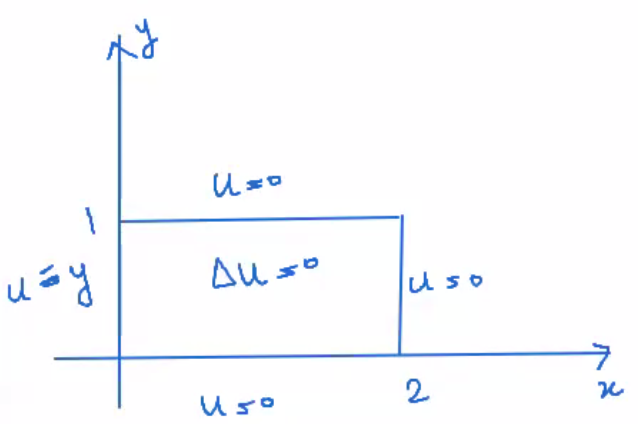
\includegraphics[width = 0.6 \textwidth]{image3.png}
\end{center}

$$u_w (x,y) = X(x) Y(y)$$

$$\frac{X''}{X} = - \frac{Y''}{Y} = \lambda$$

Problem for $Y(y): Y'' + \lambda Y = 0$. Given that $Y(0) = 0$ and $Y(1) = 0$, this is a P1 problem. 

$$\Rightarrow \lambda_n = (n \pi)^2, \quad Y_n(y) = \sin(n \pi y)$$

Solve for $X(n)$:

$$X'' - (n \pi)^2 X_n = 0 \Rightarrow X_n (x) = C_1 e^{n \pi x} + C_2 e^{-n \pi x}$$

Given that $X(2) = 0$:

$$\Rightarrow X_n (x) = C_1 \left[ e^{n \pi x} - e^{- n \pi (x-4)} \right] = 2 C_1 e^{2 n \pi} \left[ \frac{e^{n \pi (x-2)} - e^{- n \pi (x-2)}}{2} \right]$$

As a result, 

$$\Rightarrow X_n (x) = d_n \sinh \left( n \pi (x-2) \right)$$

$$\Rightarrow u(x,y) = \sum_{n=1}^\infty d_n \sinh \left( n \pi (x-2) \right) \sin (n \pi y)$$

Inhomogeneous boundary condition: $u(0,y) = y$

$$y = - \sum_{n=1}^\infty d_n \sinh \left( 2 n \pi \right) \sin (n \pi y)$$

Write a Fourier sine series for $f_w(y) = y = \sum_{n=1}^\infty b_n \sin (n \pi y)$

$$b_n = 2 \int_0^1 y \sin(n \pi y) \ud y = \left. -2y \frac{\cos(n \pi y)}{n \pi} \right|_0^1 + \underbrace{\int_0^1 \frac{2}{n \pi} \cos(n \pi y) \ud y}_{ = 0} = \frac{-2}{n \pi} (-1)^n$$

Matching coefficients:

$$- d_n \sinh (2 n \pi) = \frac{2 (-1)^{n+1}}{n \pi} \Rightarrow d_n = \frac{2 (-1)^n}{n \pi \sinh(2 n \pi)}$$

Finally, the solution is the following:

$$\Rightarrow u(x,y) = \sum_{n=1}^\infty \frac{2 (-1)^{n}}{n \pi} \frac{\sinh(n \pi (x-2))}{\sinh (2 n \pi)} \sin(n \pi y)$$

\subsubsection{A few quick notes}

\begin{itemize}
    \item $\sinh(x)$ is odd, meaning $- \sinh(x) = \sinh(-x)$
    \item However, $\cosh(x)$ is even, meaning $\cosh(x) = \cosh(-x)$
    \item $\sinh(0) = 0$
    \item $\cosh(0) = 1$
\end{itemize}

In general,

$$u_w(x,y) = -\sum_{n=1}^\infty d_n \frac{\sinh( \frac{n \pi}{b} (x-a))}{\sinh( \frac{n \pi}{b} a)} \sin( \frac{n \pi}{b} y)$$

Exercise:

$$u_E (x,y) = \sum_{n=1}^\infty a_n \frac{\sinh ( \frac{n \pi x}{b})}{ \sinh( \frac{n \pi a}{b})} \sin( \frac{n \pi y}{b})$$

\begin{center}
    $a_n$ = Fourier sine series coefficients for $f_E (y)$
\end{center}

Exercise:

$$u_N (x,y) = \sum_{n=1}^\infty C_n \frac{ \sinh( \frac{n \pi y}{a})}{\sinh( \frac{n \pi b}{a})} \sin ( \frac{n \pi x}{a})$$

$$C_n = \frac{2}{a} \int_0^a f_N (x) \sin( \frac{n \pi x}{a}) \ud x$$

The above is the Fourier sine series coefficient for north function ($f_n$). 

South:

$$u_s (x,y) = - \sum_{n=1}^\infty b_n \frac{\sinh( \frac{n \pi}{a} (y-b))}{\sinh ( \frac{n \pi b}{a})} \sin( \frac{n \pi x}{a})$$

where $b_n$ = FSS coefficients for $f_s(x)$

\subsection{Example 14}

Outline how you would solve the following boundary value problem:

$$\Delta u = 0, \begin{matrix} 0 < x < \underbrace{3}_{=a} \\ 0 < y < \underbrace{2}_{=b} \end{matrix}$$

$$u(0,y) = 0, \quad u(3,y) = \sin(\pi y)$$

$$u(x,0) = x, \quad u(x,2) = 0$$

Divide into blocks. 

\begin{center}
    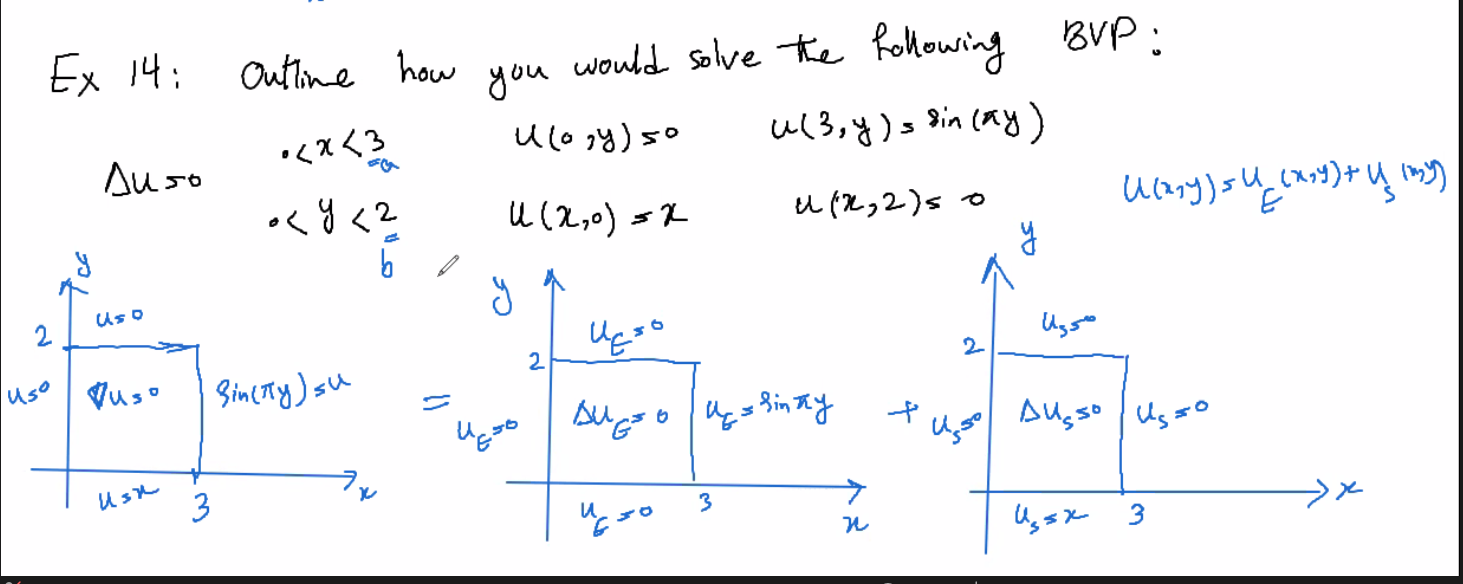
\includegraphics[width = 0.9 \textwidth]{image7.png}
\end{center}

$$u(x,y) = u_E (x,y) + u_S (x,y)$$

East boundary value problem:

FSS (Fourier sine series) for $\sin(\pi y)$:

$$\sin( \pi y) = \sum_{n=1}^\infty b_n \sin( \frac{n \pi}{2} y)$$

For any $n$ value other than 2, $b_n = 0$. 

The solution is $n = 2$, with $b_2 = 1$

$$u_E (x,y) = \frac{\sinh ( \pi x)}{\sinh (3 \pi)} \sin(\pi y) \quad (n = 2)$$

South BVP:

$$x = \sum_{n=1}^\infty b_n \sin( \frac{n \pi}{3} x)$$

$$b_n = \frac{2}{3} \int_0^3 x \sin( \frac{n \pi}{3} x) \ud x = \left. \frac{2}{3} \left( - \frac{3}{n \pi} x \cos( \frac{n \pi}{3} x) \right|_0^3 + \frac{3}{n \pi} \int_0^3 \cos( \frac{n \pi}{3} x) \ud x \right)$$

%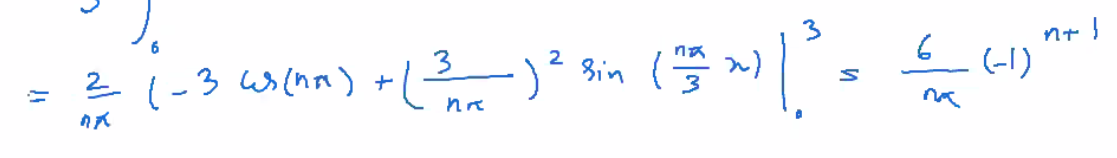
\includegraphics[width = 0.7 \textwidth]{image6.png}

$$ = \frac{2}{n \pi} \left(-3 \cos(n \pi) + ( \frac{3}{n \pi})^2 \left. \sin( \frac{n \pi}{3} x) \right|_0^3 \right)= \frac{6}{n \pi} (-1)^{n + 1}$$

$$u_x(x,y) = \sum_{n=1}^\infty \frac{6 (-1)^{n+1}}{n \pi} \frac{ \sinh( \frac{n \pi}{3} (y-2))}{\sinh( \frac{2 n\pi}{3})}  \sin( \frac{n \pi}{3} x)$$

Finally, we have the following:

$$u(x,y) = u_E (x,y) + u_S (x,y)$$




\end{document}